(Thanks to Liam for helping out on this section)
\section{Regular Expressions}
\subsection{Regular Language}
Strings can be broken down as "regular expressions", a logical expression that can be used to solve matching and searching problems. A matching problem can be checking if a string is a valid password that contains at least $X$ characters and at least $Y$ digits. A searching problem can be, given a string, list all occurrences of an email address in it. Regexps are used to solve problems like these.

For example, the regular expression \textbf{c(bb$|$ca)$^*$} will return true when matched with \textbf{cbbbbca} but return false when matched with \textbf{bca}. To solve problems using regexps, we can use Deterministic Finite Automatons (DFAs). They are deterministic because the initial state and the result of each transition are specified, and finite because there set of states is a finite set. When given a string, in the DFA seen, it will process each letter one at a time, going from state and following the transitions.

\begin{figure}[!htb]
	\center{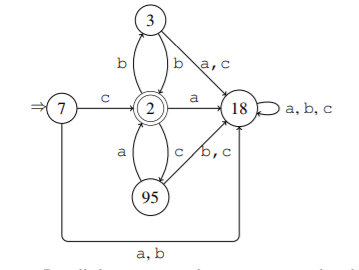
\includegraphics[width=8cm]
		{models/dfa}}
	\caption{\label{fig:dfa} Example of a DFA}
\end{figure}

As you can see, there are a few loops/areas where the DFA will definitely return false once it reaches a certain point. A more efficient way to deal with these things is to completely remove the transitions, and have it return a failure at points we know it will definitely fail. These are called partial DFAs, denoted by the $\delta$ symbol ($\delta$DFA). These are usually faster to write and run faster.

What happens when the DFA is not deterministic? An NFA if you will. NFAs differ from DFAs in two ways.
\begin{itemize}
	\item An NFA can have several initial states
	\item From a given state, when $a$ is input, there can be several possible next states.
\end{itemize}
NFAs are a relation and not a function. They can still return acceptable words, but a program can make no use of it since its, well, non-deterministic. However, there are ways to determinize an NFA. The best, basic way to accomplish this is to combine states into a set of state transitions if they match similar inputs/outputs. Conversion can take a few steps, but it's fairly simple and systematic in this regard.

Some trouble can pop up from NFAs with an $\epsilon$ transition, or an empty transitions. These bad boys can change from one state to another for literally no reason. These NFAs are called $\epsilon$NFAs, which seems obvious. With this out of the way, let's make note of Kleene's Theorem. \textbf{For a language $L$, the following are equivalent:}
\begin{itemize}
	\item L is regular
	\item The matching problem for L can be solved by a DFA.
\end{itemize}

A systematic way to turn a regexp to an equal DFA:
\begin{enumerate}
	\item Convert the regexp into an $\epsilon$NFA
	\item Convert it down to an NFA
	\item Convert it further down to a DFA.
	\item Minimize DFA size by identifying equivalent states, removing unreachable states and just general refactoring.
\end{enumerate}
\subsection{Non-regular Language}
We know that some languages are not regular, because there are uncountably many languages and only countably many regexps. An example of a useful non-regular language is the language of well-balanced brackets. The check for balance can be done in a stack, pushing and popping from a stack when reading '(' and ')' respectively. However, if we have a large amount of '(', the stack will overflow thanks to our finite memory.
\begin{figure}[!htb]
	\center{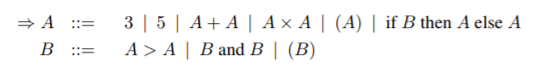
\includegraphics[width=14cm]
		{models/bnf}}
	\caption{\label{fig:dfa} Example of a BNF}
\end{figure}
When talking about non-regular languages, we can talk about context-free grammars. Grammars are written in Backus-Naur Form (BNF) and, in basic terms, represent different characters as symbols and use these symbols to derive a word. These symbols are either terminal or non-terminal; terminal means it can be expanded to a final value of sorts. The grammars we covered are context-free because you can apply a production rule to any non-terminal regardless of the other symbols in the word.
\begin{figure}[!htb]
	\center{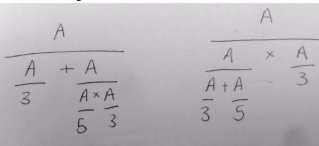
\includegraphics[width=7cm]
		{models/derivationtree}}
	\caption{\label{fig:dfa} Ambiguous derivation tree}
\end{figure}
\paragraph{Some Definitions}
\begin{itemize}
	\item Leftmost Derivation: Converting a grammar to a word by replacing the leftmost non-terminal
	\item Derivation Tree: A tree structure representing a derived word where each leaf is a non-terminal.
	\item Ambiguous: A grammar is ambiguous when there is more than 1 derivation tree possible with left-most derivation
\end{itemize}
\section{Turing Machines}
\subsection{Turing Machines}
A turing machine is the precise model of computation (roll credits) that are used to determine decidability and complexity of programs. A turing machine has finitely many states, but it also has access to an external, infinite memory in the form of a tape. The machine has a head that sits over one of the cells in a tape. A concise definition of the turing machine consists of the following data:
\begin{itemize}
	\item A finite state X of states
	\item An initial state p
	\item A transition function $\delta$ from X to:
	\begin{enumerate}
		\item Read
		\item Write
		\item Left
		\item Right
		\item No-op
		\item Return
	\end{enumerate}
\end{itemize}
There are also a few variants that expand on the basic turing machine.
\paragraph{Auxiliary Characters} In addition to the input alphabet and "blank", a turing machine can have auxiliary characters that are used during the completion of a program, but these characters cannot appear at the start or at the end of a task.
\paragraph{Auxiliary Tape} A two-tape Turing Machine has, well, two tapes. A program is now capable of completing tasks that read/write etc. on two tapes (Main x, Aux x). The copy-reverse problem can be solved in linear time using a two-tape machine. 
\paragraph{2D Turing Machine} Instead of a tape, a 2D machine has a sheet instead of a tape, so it can go up and down. It must ensure that all but one row are blank on completion of a program.
\section{Complexity}
\subsection{Complexity of Programs}
When trying to find the number of steps, it is helpful to remember some laws of summations. The most important part of complexity for our course is to practice deriving worst case and average case complexities.
\begin{figure}[!htb]
	\center{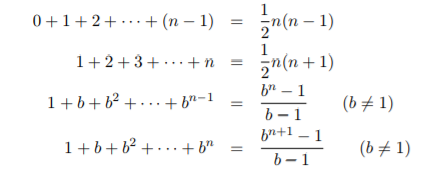
\includegraphics[width=12cm]
		{models/sums}}
	\caption{\label{fig:sum} Helpful sums to memorize}
\end{figure}
Hopefully you remember how Big O worked from Year 1 DSA. There's a bit more in Models than what we learned, a more interesting way of deriving it. \[\exists M. \exists C. \forall n \geq M. f(n) \leq C \times g(n)\]
$M$ is an arbitrary number. The set from $n = [M, +\inf]$ will hold true.

There is one more variation to this for polynomial complexity. Polynomial time solutions are said to be \textit{feasible}. 
\[\exists M. \exists C. \exists k. \forall n \geq M. f(n) \leq C \times n^k\]
\subsection{P and NP}
\paragraph{Definitions}
\begin{itemize}
	\item Search Problem: Relation from the set of words (problems) to the set of words (solutions).
	\item $NP$ Search Problem: Search problems with solution of polynomial size and checked in polynomial time. Will have a solution in exponential time.
\end{itemize}
What is the NP = P problem? It is the question, can every NP search problem be solved in polynomial time?  If  the  answer is  yes  for Sudoku,  then  it’s yes  for every NP search problem.  This is because Sudoku is a special kind of NP search problem called “NP-complete”, meaning that it’s as hard as an NP search problem can be. Any NP search problem can be reduced (in polynomial time) to Sudoku. By contrast, it is not known whether factorization is NP-complete, so showing that factorization can be solved in polynomial time won’t prove anything major.
\subsection{NP-Completeness}
\paragraph{SAT} A problem instance of this NP search problem consists of propositional variables and a formula built from this variables. The formulas are generated from a specific grammar. A satisfying assignment is an assignment of truth variables that makes the formula true. SAT is useful in solving constraint problems, like "I need to study Models with Jon and I need to study Security with Clair, but all of our free times can only coincide once." You can use SAT to potentially find the magic timings.
\paragraph{Cook's Theorem} Any NP problem can be reduced to SAT, like $n$Sudoku for example. Find a mapping of different characters and constraints to propositional logic, and you have reduced your problem to SAT.
\section{Decidability}
A decision problem is said to be decidable when there is some program that, when given an argument, says whether the answer is Yes/No.
\subsection{Reduction and Decidability}
\paragraph{Church's Thesis} Any decision problem on words that can be solved by an algorithm can be solved by a Turing machine.
\paragraph{Reduction}
Suppose we have two problems P and Q. Suppose that we show how to solve Q using a black box that solves P. Then is called reducing problem Q to problem P. 
For example, I saw a recipe for profiteroles that said “take some pastry balls” and “take some chocolate sauce”. The author reduced the problem of making profiteroles to the problems of making pastry balls and making chocolate sauce. 
Suppose we’ve reduced problem Q to problem P. 
\begin{itemize}
	\item If P is decidable, then Q is decidable
	\item If Q is undecidable, then P is undecidable
\end{itemize}
\paragraph{Halting Problem}
Some programs run forever, others halt. Usually we want our programs to halt; if they run forever, that’s a bug. Can we test this automatically? Our main man Turing proved the halting problem to be undecidable. We begin the proof by assuming it is decidable. Consider the unary halting problem: given a unary Java method.
\begin{verbatim}
void f(String x) {
    ...
}
\end{verbatim}
and a String $y$, does $f$ terminate when called with argument y? We can reduce this problem to a nullary one.
Take the code of $f$ and replace $x$ with $y$; then the nullary method ($g$) terminates when called if $f$ terminates when called with argument $y$. Since the nullary problem is, on assumption, decidable, the unary one is too. So we have a program:
\begin{verbatim}
boolean haltcheck(String somemethod, String y)
\end{verbatim}
Where $somemethod$ is the body of a unary method. When applied to $M$ and $y$, this method returns true if $M$ applied to $y$ terminates, otherwise it returns false.\newline
2. Next, we turn this into a program.
\begin{verbatim}
hangcheck(String somemethod, String y) {
    if haltcheck(somemethod, y) {
        while (true) {}
    } else {
        return;
    }
}
\end{verbatim}
This method, when applied to M and y, hangs if M and applied to y terminates, otherwise it returns.\newline
3. Next, we turn this into a program:

\begin{verbatim}
void doublehang(String y) {
    hangcheck(y,y);
}
\end{verbatim}
This method, when applied to $y$ (the body of a unary method), will hang if $y$ applied to $y$ terminates, otherwise it returns.\newline
4. Finally let $z$ be the body of $doublehang$. We see that $doublehang$, when applied to $z$, terminates if it hangs. Contradiction. (Objection!)
\paragraph{Semantics} Semantic properties of a code are properties that affect the behaviour of the program. For example, does this software only print polite words? Does this software, when supplied with two positive integers, always return the highest common factor? Surprise surprise, we can't. Thanks to our good friend from down the tape, Rice's Theorem states that, in all but two cases, every semantic property is undecidable. That's because there are three cases, and Rice only covers the third one, since the other two are decidable.
\begin{enumerate}
	\item A property never holds (decidable)
	\item A property always holds (decidable)
	\item A property sometimes holds and sometimes doesn't (Undecidable due to Rice's Theorem) 
\end{enumerate}
\section{Lambda Calculus}
\paragraph{Conventions}  $\lambda x$ is equivalent to \textbf{fun x $\rightarrow$} in OCaml. Just a quick convention comparison to get you up to speed. 
\begin{itemize}
	\item Juxtaposition is application
	\item Application has highest precedence
	\item $\lambda x$ has lowest precedence
	\item Arithmetic Operations are intermediate
	\item Application associates to the left ($M N P$ is bracketed as $(M N) P$ not as  $M (N P)$)
\end{itemize}
\begin{figure}[!htb]
	\center{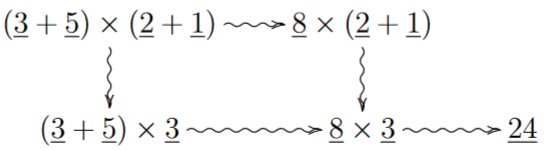
\includegraphics[width=8cm]
		{models/reduction}}
	\caption{\label{fig:reduct} Reduction Graph with more than one order}
\end{figure}
\subsection{Reduction and Equivalence}
There are two types of reduction, $\delta$-reduction and $\beta$-reduction.
\begin{itemize}
	\item $\delta$-reduction: Basic arithmetic reduction ($m x n \rightarrow mn$)
	\item $\beta$-reduction: Applies $\lambda$-abstractions (($\lambda x.x + 3)7 \rightsquigarrow_{\beta}$ (7 + 3))
\end{itemize}
We use a combination of both to formulate reduction graphs. Reduction can branch of and be done in different evaluation orders, as seen in the figure. There is also the notion of $\alpha$-equivalence, which is simply when two lambda function evaluate to the same result despite being different originally.
